%%%%%%%%%%%%%%%%%%%%%%%%%%%%%%%%%%%%%%%%%
% Original author:
% Linux and Unix Users Group at Virginia Tech Wiki
% (https://vtluug.org/wiki/Example_LaTeX_chem_lab_report)
% Modified by: Hector F. Jimenez S, for the Digital Electronics Laboratory.
% License:
% CC BY-NC-SA 3.0 
%%%%%%%%%%%%%%%%%%%%%%%%%%%%%%%%%%%%%%%%%
%----------------------------------------
%   PACKAGES AND DOCUMENT CONFIGURATIONS
%---------------------------------------
\documentclass[paper=a4, fontsize=12pt]{article}        % A4 paper and 11pt font size
\usepackage[T1]{fontenc}                                % Use 8-bit encoding that has 256 glyphs
%\usepackage{fourier}                                   % Use the Adobe Utopia font for the document 
\usepackage[spanish,english]{babel}                     % Spanish Language, templates uses some sections in english.
\selectlanguage{spanish}                                % main language.
\usepackage{subfig}
\usepackage{multirow}
\PassOptionsToPackage{spanish}{babel}
\renewcommand{\figurename}{Figura}                      % Force rename of figure.
\renewcommand{\figurename}{Fig.}
\usepackage[figurename=Fig.]{caption}
\usepackage[utf8]{inputenc}                             % tildes for spanish language.
\usepackage{amsmath,amsfonts,amsthm}                    % Math packages.
\usepackage{minted}                                     % For syntax highlighting.
        \renewcommand\listingscaption{Código}           %rename the source code minted !
\usepackage{float}                                      % Image will be in the same place as you want.!!! x-/
\usepackage{sectsty}                                    % Allows customizing section commands
\allsectionsfont{\centering \normalfont\scshape}        % Make all sections centered, the default font and small caps
\usepackage{hyperref}
\hypersetup{                                            %Setups the false color and borders.
    colorlinks=false,
    pdfborder={0 0 0},
}
\newcommand\fnurl[2]{%                                  % set a simple and quick footnote command and include url.
\href{#2}{#1}\footnote{\url{#2}}%   
}
\usepackage{graphicx}                                   % Import easyly images.
\graphicspath{ {./images/} }                            % Where to look for the images.
\DeclareGraphicsExtensions{.pdf,.png,.jpg}              % Graphics Extension to be used
\usepackage[notes,backend=biber]{biblatex-chicago}      % Bibliography and references.
\bibliography{biblio}                                   % bibliography filename.
\usepackage{fancyhdr}                                   % Custom headers and footers
\pagestyle{fancyplain}                                  % Makes all pages in the document conform to the custom headers and footers
\fancyhead{}                                            % No page header
\fancyfoot[L]{}                                         % Empty left footer
\fancyfoot[C]{}                                         % Empty center footer
\fancyfoot[R]{\thepage}                                 % Page numbering for right footer
\renewcommand{\headrulewidth}{0pt}                      % Remove header underlines
\renewcommand{\footrulewidth}{0pt}                      % Remove footer underlines
\setlength{\headheight}{13.6pt}                         % Customize the height of the header
\numberwithin{equation}{section}                        % Number equations within sections (i.e. 1.1, 1.2, 2.1, 2.2 instead of 1, 2, 3, 4)
%\numberwithin{figure}{section}                         % Number figures within sections (i.e. 1.1, 1.2, 2.1, 2.2 instead of 1, 2)
\numberwithin{table}{section}                           % Number tables within sections (i.e. 1.1, 1.2, 2.1, 2.2 instead of 1, 2, 3, 4)
\setlength\parindent{0pt}                               % Removes all indentation from paragraphs
\newcommand{\horrule}[1]{\rule{\linewidth}{#1}}         % Create horizontal rule command with 1 argument of height
\usepackage{listings}% http://ctan.org/pkg/listings
\usepackage{multicol}
\usepackage{caption}
\usepackage{subfig}
\renewcommand{\lstlistingname}{Código}  
\title{Sistemas Operativos I\\ 
\horrule{0.5pt} \\[0.4cm]                               % Thin top horizontal rule  Title rule
\textit{Taller 5: Caso de estudio del sistema operativo Unix System V, Release 4}
\horrule{1pt} \\[0.5cm]             
}           

\author{                                                
Héctor F. \textsc{Jiménez Saldarriaga.}\\               % Authors begin.
\texttt{hfjimenez@utp.edu.co} \\                        
\texttt{PGP KEY ID: 0xB05AD7B8}
} 
% End of  Author name
\date{}                                                % Date for the report, this will hide the \today.

\begin{document}
\maketitle                                             % Insert the title, author and date
\begin{center}
\begin{tabular}{l r}                                   % two column to
Fecha de Entrega: & Marzo, 2018 \\                 % Ramiro's Details.
Profesor: & Cesar Manuel Castillo Rodriguez
\end{tabular}
\end{center}
%%%%%%%%%%% 
% Let's start the document.
%%%%%%%%%%% 
\section{Objetivos}
\begin{itemize}
    \item Evolución
    \item Realizar el proceso de instalación del sistema operativo  
    \item Identificar el manejo de Archivos, Shell
    \item Estructura del Sistema Operativo
    \item Clasificación del Sistema Operativo
    \item Ejecución de Comandos, al menos 25.
\end{itemize}
\section{Evolución de Unix} 
System V Unix ó Unix System V, comúnmente abreviado \textbf{\textit{SysV}} y rara vez se llama Sistema de Mayo, fue una de las versiones del sistema operativo Unix.Fue desarrollado originalmente por AT \& T y lanzó por primera vez en 1983.  Cuatro versiones del Sistema V fueron puestos en libertad, calificó los módulos 1, 2, 3 y 4 como las versiones más exitosas. La fuente de Unix posee varias características comunes, tales como los \textit{Sys V init scripts} (\textbf{/etc/init.d}), que se usan para controlar el sistema de arranque y cierre de todos los servicios.

El sistema también constituye la base de la definición de interfaz System V (SVID), un estándar de la definición de la forma en que el sistema V tienen acuerdos de trabajo. El otro de los dos principales ramas del sistema Unix es Berkeley Software Distribution. Mientras que AT \& T vendió su propio hardware que se desarrolló del Sistema V (véase el AT \& T en Informática de Sistemas), la mayoría de los clientes corrió una versión de un distribuidor, sobre la base de AT \& T de referencia de aplicación.
Según también el articulo presentado en \fnurl{Wikipedia}{https://en.wikipedia.org/wiki/UNIX_System_V}
Esta liberacion 4 tenia varias caracteristicas y mejoras importantes entre ellas : 
\begin{itemize}
\item Soporte TCP/IP, sockets, UFS, soporte para múltiples grupos,  shell escrita en C, todo ella obtenida de BSD.
\item Implementacion de una interfaz para el sistema de archivos virtual, Soporte de NFS.
\item Mejora de compatibilidad para utilización de librerías compartidas en el sistemas.
\item  Implementacion de OpenWindows Gui para entornos gráficos.
\item Soporte multilenguaje gracias al paquete MNLS.
\item Soporte para el estándar POSIX y X/Open.
\end{itemize}
Para realizar el proceso de instalación de SysVR4 lo que se hizo fue seguir el tutorial provisto del profesor, en este tutorial se explica en detalle como realizar la instalación del sistema operativo base, sus componentes y paquetes externos y drivers para el sistema. Desafortunada-mente, el sistema no explica como realizar la instalación del sistema  gráfico. 
$$\\$$
\section{Proceso de instalación Unix System V R4}
\begin{figure}[H]
    \centering
    \subfloat[Bienvenida Instalador Unix System V R4]{\label{fig:bienvenida}{
        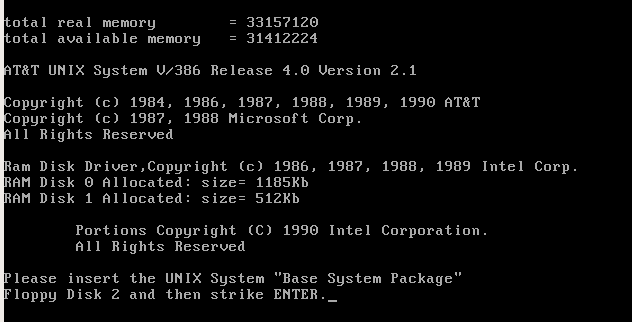
\includegraphics[width=0.68\textwidth]{img/2.png}
        }}
    \subfloat[Aceptando terminos de instalacion de Unix]{\label{fig:formateada}{
        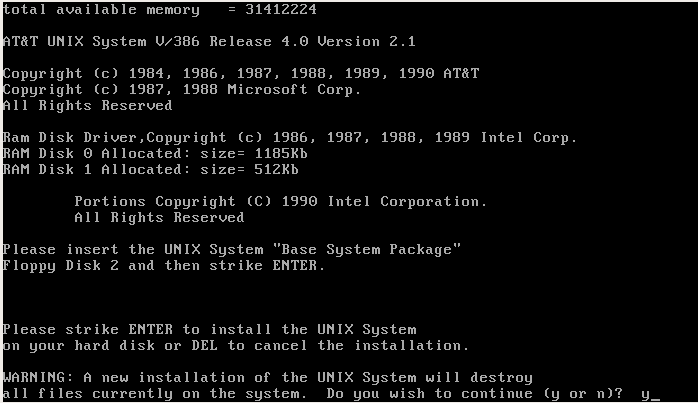
\includegraphics[width=0.68\textwidth]{img/3.png}
        }}
       \hfill
    \subfloat[Utilizaremos 100\% del disco  para la instalacion.]{\label{fig:disco}{
        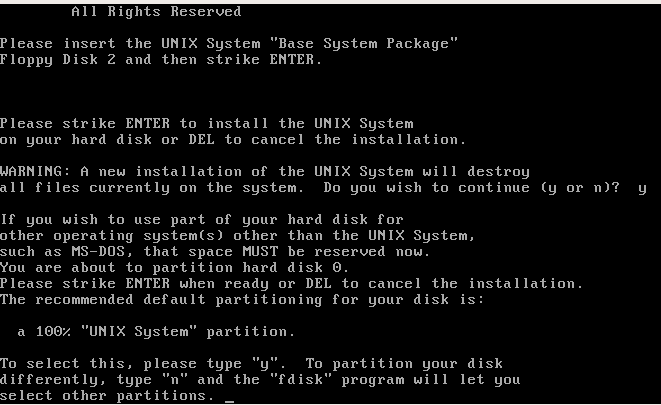
\includegraphics[width=0.68\textwidth]{img/4.png}
        }}
    \subfloat[Seleccion  del Sistema de Archivos para la Instalacion\textit{ufs}]{\label{fig:ufs}{
        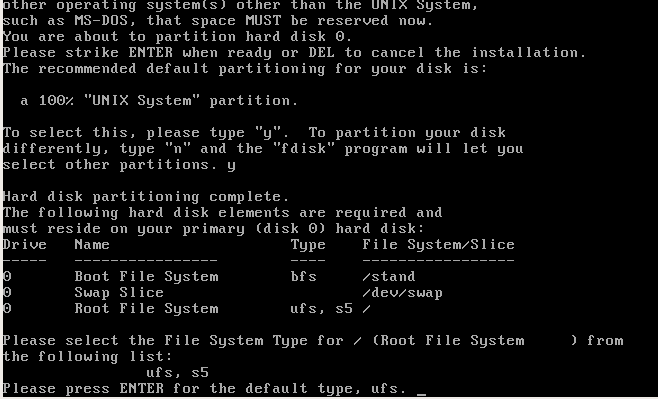
\includegraphics[width=0.68\textwidth]{img/5.png}
        }}
        \hfill
    \subfloat[Confirmación de particiones y ubicación de instalación.]{\label{fig:confirmar}{
        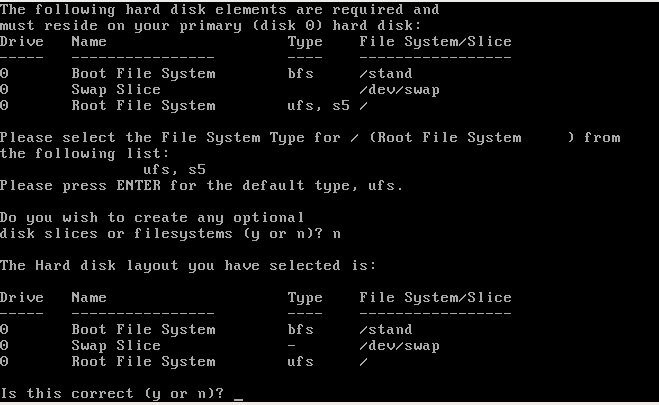
\includegraphics[width=0.68\textwidth]{img/6.png}
        }}
    \subfloat[El sistema decide los tamaños para las particiones.]{\label{fig:particiones}{
        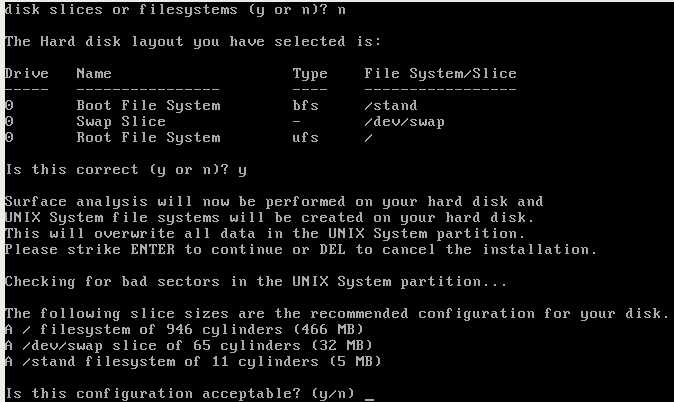
\includegraphics[width=0.68\textwidth]{img/7.png}
        }}
    \caption{Configuración inicial de instalación}
\end{figure}

\begin{figure}[H]
    \centering
    \subfloat[]{\label{fig:bienvenida}{
        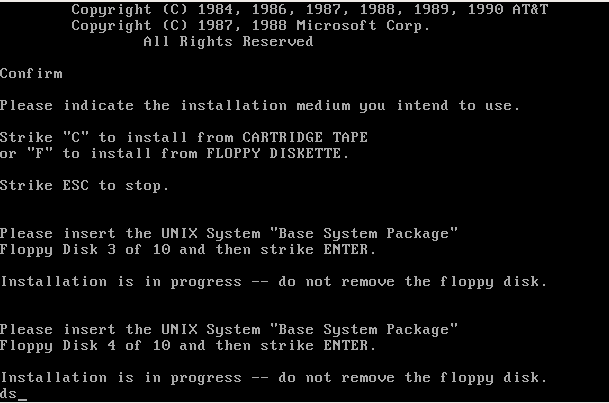
\includegraphics[width=0.68\textwidth]{img/8.png}
        }}
    \subfloat[]{\label{fig:formateada}{
        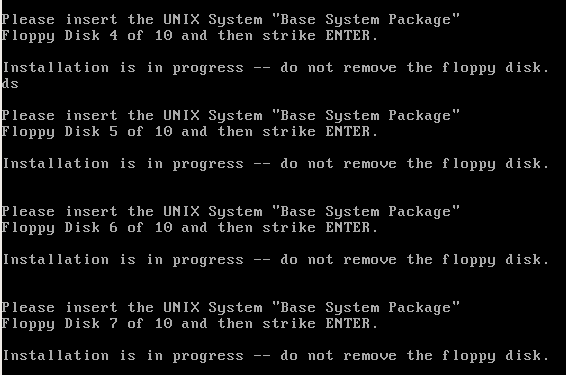
\includegraphics[width=0.68\textwidth]{img/9.png}
        }}
       \hfill
    \subfloat[]{\label{fig:disco}{
        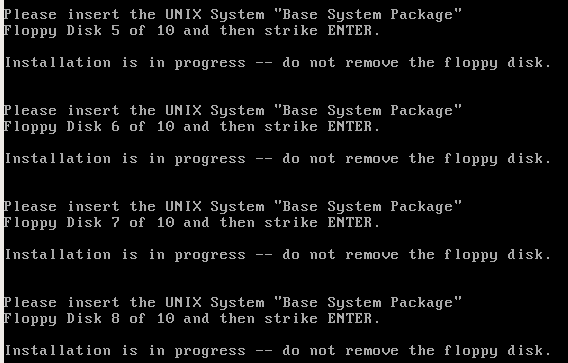
\includegraphics[width=0.68\textwidth]{img/10.png}
        }}
      \subfloat[Ultimo Diskette 10 de 10]{\label{fig:ufs}{
        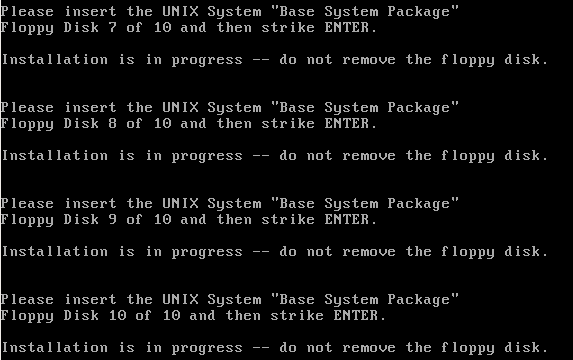
\includegraphics[width=0.68\textwidth]{img/11.png}
        }}
    \caption{Proceso secuencial de instalación, intercambio de diskettes}
\end{figure}

\begin{figure}[H]
    \centering
    \subfloat[Configuracion Inicial de usuarios del sistema \textit{root, install, service}]{\label{fig:bienvenida}{
        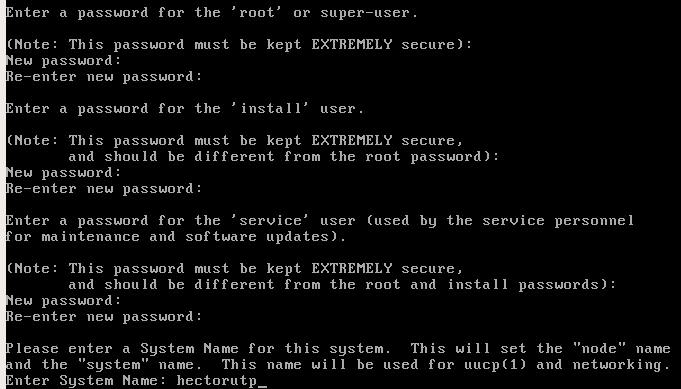
\includegraphics[width=0.68\textwidth]{img/12.png}
        }}
    \subfloat[Logueo exitoso al sistema usando la cuenta de root]{\label{fig:formateada}{
        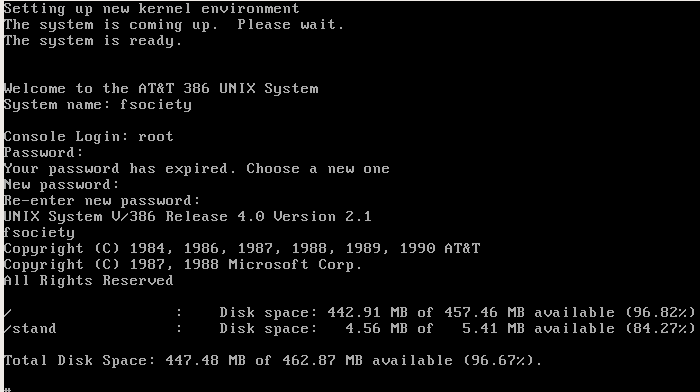
\includegraphics[width=0.68\textwidth]{img/13.png}
        }}
       \hfill
    \subfloat[Instalacion de paquetes, OA\&M]{\label{fig:disco}{
        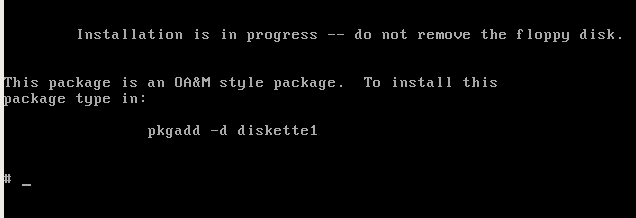
\includegraphics[width=0.68\textwidth]{img/14.png}
        }}
    \subfloat[Instalacion de paquetes, OA\&M y licencia para mas de 16 usuarios]{\label{fig:ufs}{
        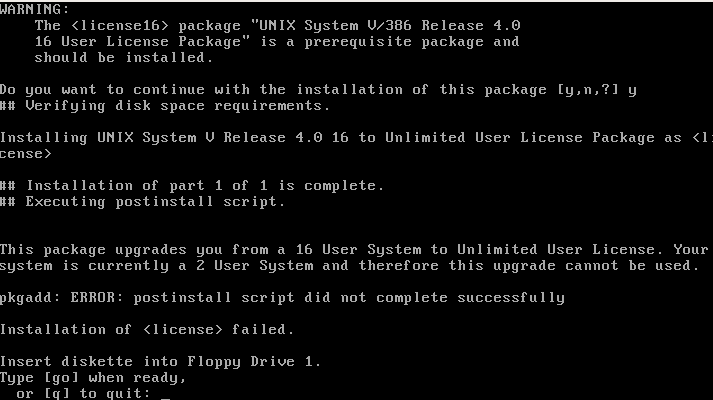
\includegraphics[width=0.68\textwidth]{img/15.png}
        }}
        \hfill
    \subfloat[Instalacion de Paquetes Xenix, Drivers y pseudo dispositivos]{\label{fig:confirmar}{
        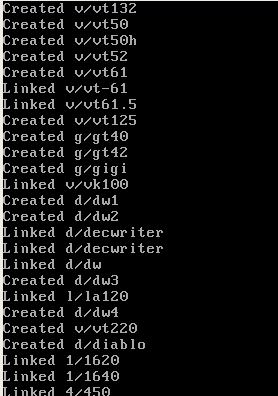
\includegraphics[width=0.56\textwidth]{img/16.png}
        }}
    \subfloat[Instalacion del software de compatibilidad BSD]{\label{fig:particiones}{
        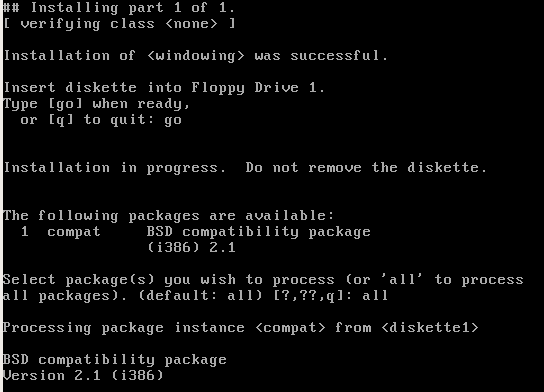
\includegraphics[width=0.68\textwidth]{img/17.png}
        }}
    \caption{Instalacion de paquetes y software extra en el sistema.}
\end{figure}


\begin{figure}[H]
    \centering
    \subfloat[Instalacion de Paquete Extra, Framed Access Command Enviroment]{\label{fig:bienvenida}{
        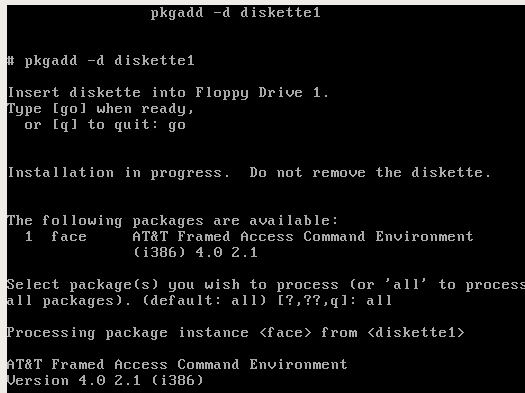
\includegraphics[width=0.68\textwidth]{img/19.png}
        }}
    \subfloat[Prueba de Soporte Extendido]{\label{fig:formateada}{
        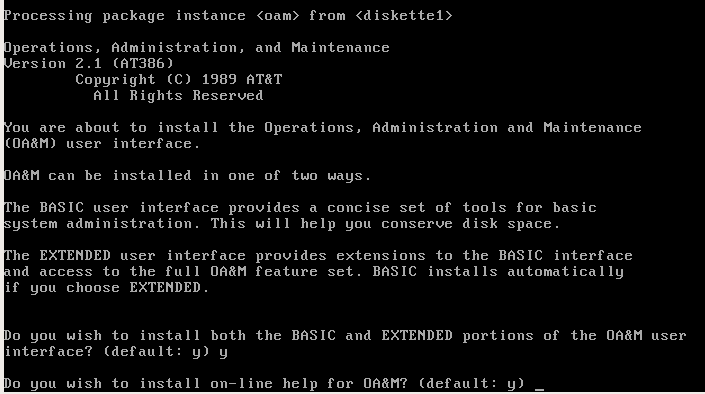
\includegraphics[width=0.68\textwidth]{img/20.png}
        }}
       \hfill
    \subfloat[Paquete de herramientas para la administracion y mantenimiento del sistema]{\label{fig:disco}{
        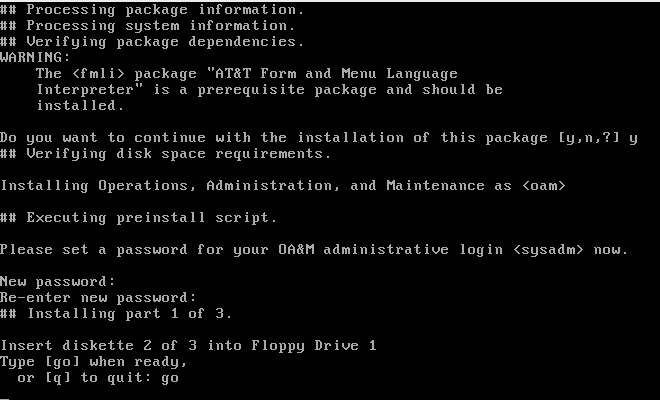
\includegraphics[width=0.68\textwidth]{img/22.png}
        }}
    \subfloat[Verificacion y pruebas de instalacion paquetes de administracion ]{\label{fig:ufs}{
        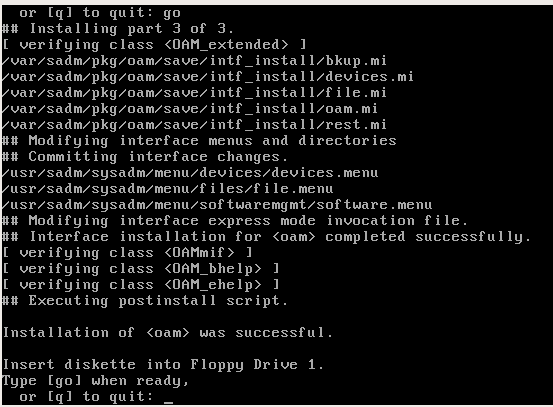
\includegraphics[width=0.68\textwidth]{img/23.png}
        }}
        \hfill
    \subfloat[Insltacion de Paquetes DFS]{\label{fig:confirmar}{
        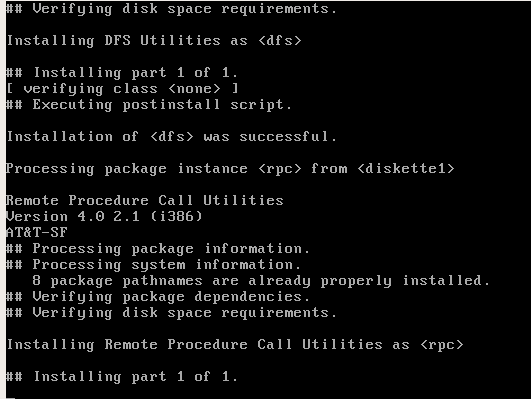
\includegraphics[width=0.68\textwidth]{img/25.png}
        }}
    \caption{Instalacion de Paquetes completa}
\end{figure}


\section{Manejo de Archivos y Estructura}
El sistema de archivos que se encuentra en este sistema operativo es de tipo jerárquico, las carpetas tiene un directorio padre, y apartir de allí tenemos un uso estándar tal cual como se encuentra documentado para el estándar POSIX. 
El Unix File System (UFS) es un sistema de archivos utilizado por varios sistemas operativos UNIX y POSIX. Es un derivado del Berkeley Fast File System (FFS), el cual es desarrollado desde FS UNIX (este último desarrollado en los Laboratorios Bell). 
\begin{center}
\begin{figure}[H]
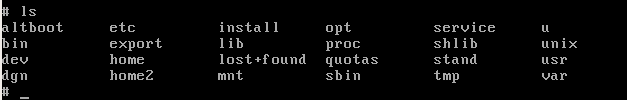
\includegraphics[scale=0.6]{img/directorios.png}
\caption{Sistema de Archivos Disponible}
\label{fig:dis2}
\end{figure}
\end{center}
Para el manejo de archivos el sistema operativo cuenta con los comandos apropiados para realizar las tareas como creacion,actualizacion,eliminacion,lectura.

\section{Ejecucion Comandos}


\begin{figure}[H]
    \centering
    \subfloat[]{\label{fig:bienvenida}{
        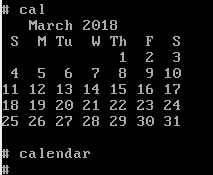
\includegraphics[width=0.68\textwidth]{img/cal.png}
        }}
    \subfloat[]{\label{fig:formateada}{
        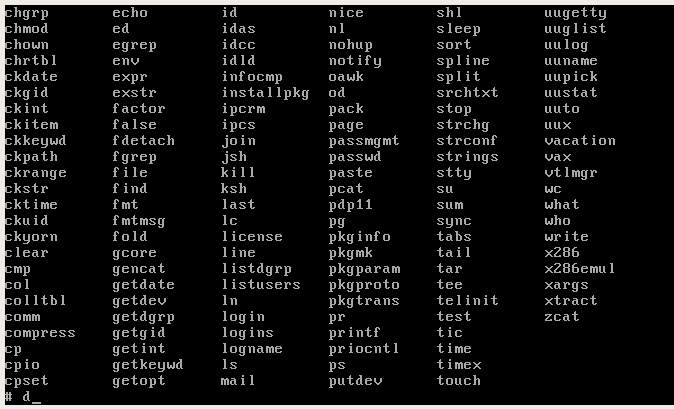
\includegraphics[width=0.68\textwidth]{img/comandos.png}
        }}
       \hfill
    \subfloat[]{\label{fig:disco}{
        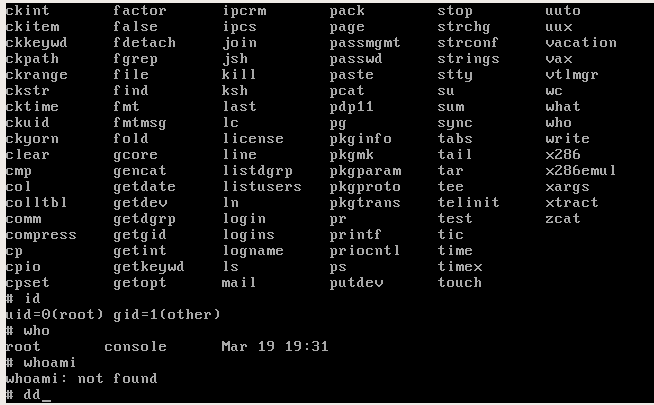
\includegraphics[width=0.68\textwidth]{img/id.png}
        }}
    \subfloat[]{\label{fig:ufs}{
        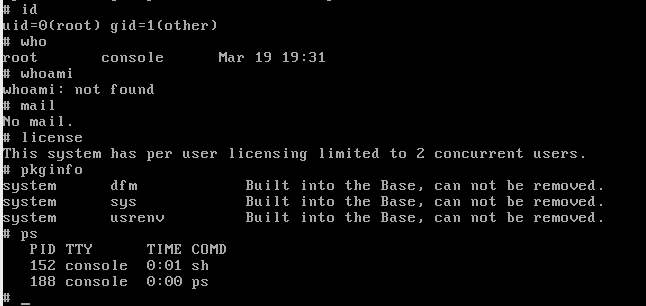
\includegraphics[width=0.68\textwidth]{img/procesos.png}
        }}
        \hfill
    \subfloat[]{\label{fig:confirmar}{
        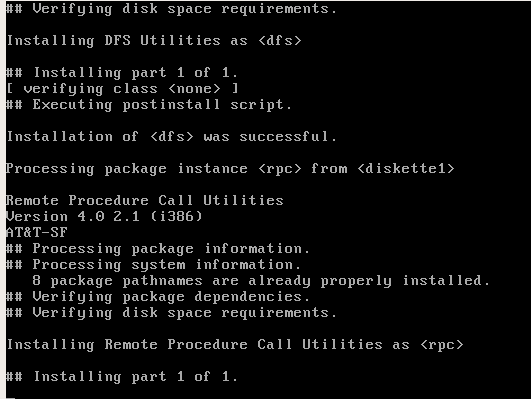
\includegraphics[width=0.68\textwidth]{img/25.png}
        }}
    \caption{Ejecución de Comandos Unix, Múltiples comandos por ventana.}
\end{figure}
Se hace uso de los siguientes comandos: 
\begin{enumerate}
  \item \textbf{vi} :Editor por defecto
\item \textbf{installpkg}: Instalación de paquetes en unix
\item \textbf{cd}: movimiento entre directorios
\item \textbf{ps}: muestra la lista de procesos en ejecución.
\item \textbf{cal}: calendario de mes.
\item \textbf{calendar}: lista actividades del cron del sistema.
\item \textbf{chown}: cambio de permisos para archivos en el sistema.
\item \textbf{mail}: muestra email recibidos por root@fsociety, donde fs.
\item \textbf{who}: identifica el usuario en uso.
\item \textbf{ls}: lista los contenidos de una carpeta.
\item \textbf{chgrp}: cambia de grupo para archivos y carpetas.
\item \textbf{date}: fecha establecida en el sistema
\item \textbf{mount}: puntos de montaje, particiones.
\item \textbf{fsck}: Verificación del sistema de archivos, revisión de bloques malos.
\item \textbf{mkdir}: Creación de carpetas.
\item \textbf{touch}: Crear archivos vacíos 
\item \textbf{cron}: Agenda miento de tareas en el sistema
\item \textbf{more}: Paginador para ver contenido de manera porcentual.
\item \textbf{adduser}: Agregar usuarios al sistema.
\item \textbf{awk}: Filtrar y procesar textos de una manera sencilla.
\begin{figure}[H]
    \centering
    \subfloat[]{\label{fig:bienvenida}{
        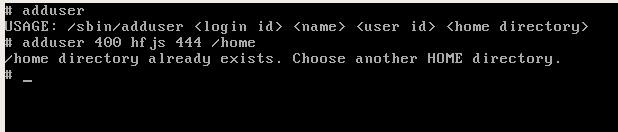
\includegraphics[width=0.68\textwidth]{img/user.png}
        }}
    \subfloat[]{\label{fig:formateada}{
        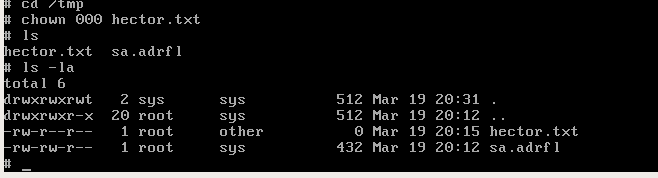
\includegraphics[width=0.68\textwidth]{img/perm.png}
        }}
       \hfill
    \subfloat[]{\label{fig:disco}{
        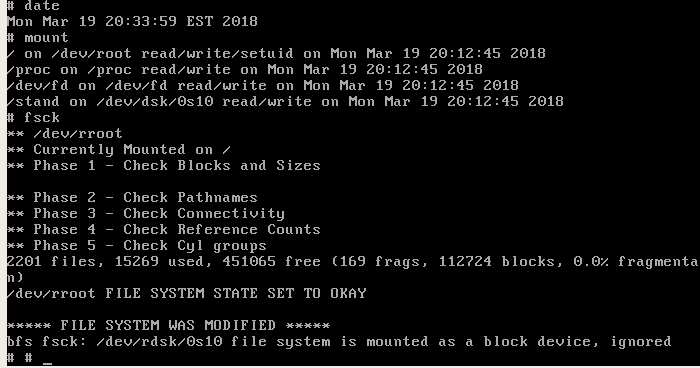
\includegraphics[width=0.68\textwidth]{img/multiples.png}
        }}
    \caption{Ejecución de Comandos Unix, Múltiples comandos por ventana.}
\end{figure}

\end{enumerate}
\section{Referencias}
\begin{itemize}
\item  \hyperref[https://www.youtube.com/watch?v=6P57ukAtCGs&spfreload=10]{Installation of Unix System V on virtualbox Youtube,  https://www.youtube.com/watch?v=6P57ukAtCGs\&spfreload=10}
\item  \hyperref[https://es.wikipedia.org/wiki/Unix_File_System]{Unix File System,  https://es.wikipedia.org/wiki/Unix-File-System}
\item  \hyperref[http://www.linfo.org/system_v.html]{System V Definition, http://www.linfo.org/system-v.html}
\end{itemize}
\end{document}